\documentclass[a4paper]{article}
\usepackage[affil-it]{authblk}

\usepackage[sort&compress]{natbib}
\usepackage[english]{babel}
\usepackage[utf8]{inputenc}
\usepackage{amsmath}
\usepackage{graphicx}
\usepackage[colorlinks,linkcolor=blue]{hyperref}
\usepackage[colorinlistoftodos]{todonotes}
\usepackage[noindent]{ctex}
\usepackage{amsmath}
\usepackage{lipsum}
\usepackage{color}
\usepackage{abstract}


\title{\Huge \heiti{Web应用英文字体分析报告}}

\author{Yuting Cao%
  \thanks{Email: \texttt{cyt12@software.nju.edu.cn}~(121250005)}} 
  \author{Jing Liu%
  \thanks{Email: \texttt{ljing12@software.nju.edu.cn}~(121250083)} }
\author{Xiaowei Miao%
  \thanks{Email: \texttt{mxw12@software.nju.edu.cn}~(121250101)}}
\affil{Software Institute, Nanjing University, Nanjing, China}

%\author{Yossi Farjoun%
%  \thanks{Electronic address: \texttt{yfarjoun@math.mit.edu}; Corresponding author}}
%\affil{G. Mill\'an Institute of Fluid Dynamics,\\ Nanoscience and Industrial
%Mathematics,\\ Universidad Carlos III de Madrid, Spain}
%\date{2015.5}
\begin{document}
\maketitle

\renewcommand{\abstractname}{摘要}

\begin{abstract}
  摘要填充。摘要填充。摘要填充。摘要填充。摘要填充。摘要填充。摘要填充。摘要填充。摘要填充。摘要填充。

  \textbf{关键字:}英文字体、Web应用、分辨率
\end{abstract}

\section{Web应用流行字体}

\subsection{总体概况}

~~~~~~1999年01月15日,Microsoft发布“TrueType core fonts for the Web”,首次提出其与Apple Inc共同研制的29种Web字型标准及其扩展版本,字型标准如Figure \ref{cyt1}所示\cite{cyt1}。

归结而言,包括:Andale Mono、Arial 、Arial Black 、Comic Sans MS、 Courier New、  Georgia、Impact、Times New Roman、Trebuchet MS、Verdana及Webdings共11类\cite{nutshell},如Figure \ref{cyt2}所示。。

\makeatletter
\def\@captype{figure}
\makeatother
\centerline{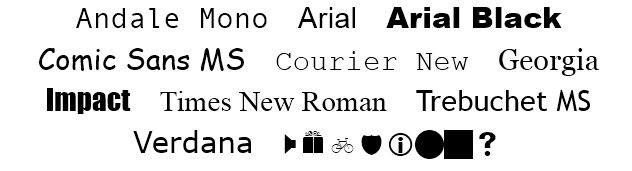
\includegraphics [width=0.8\textwidth]{cyt2.png} }
\caption{TrueType字型标准}
\label{cyt2}

当然,目前随着互联网技术的飞速发展,已有数百种Web开发字体可供选择\cite{cyt2}。相应字体的分类标准也各有不同。使用最广,对字体进行系统的分类是1954年由Maxmilien Vox制定,由Association Typographique Internationale(国际字体协会)于1962年修订的Vox-AtypI分类,将字体分为11大类\cite{cyt4},当然,这11类与TrueType归纳的11类不同。另外,法国字体艺术家Francis Thibaudeau将字体分为四大类,Antiques(sans-serif无衬线),Egyptiennes(slab-serif扁平衬线),Didots,Elzevirs(triangular serifs三角形衬线),这也是Vox分类的基础。

由于Microsoft和Apple Inc自1999年起,将其11类字型标准分别安装到Internet Explorer和Safari中,作为默认的浏览器字体为大众熟知,因而Web程序员开发大多选择这11类字体,逐渐成为当前Web主流字体。

\makeatletter
\def\@captype{figure}
\makeatother
\centerline{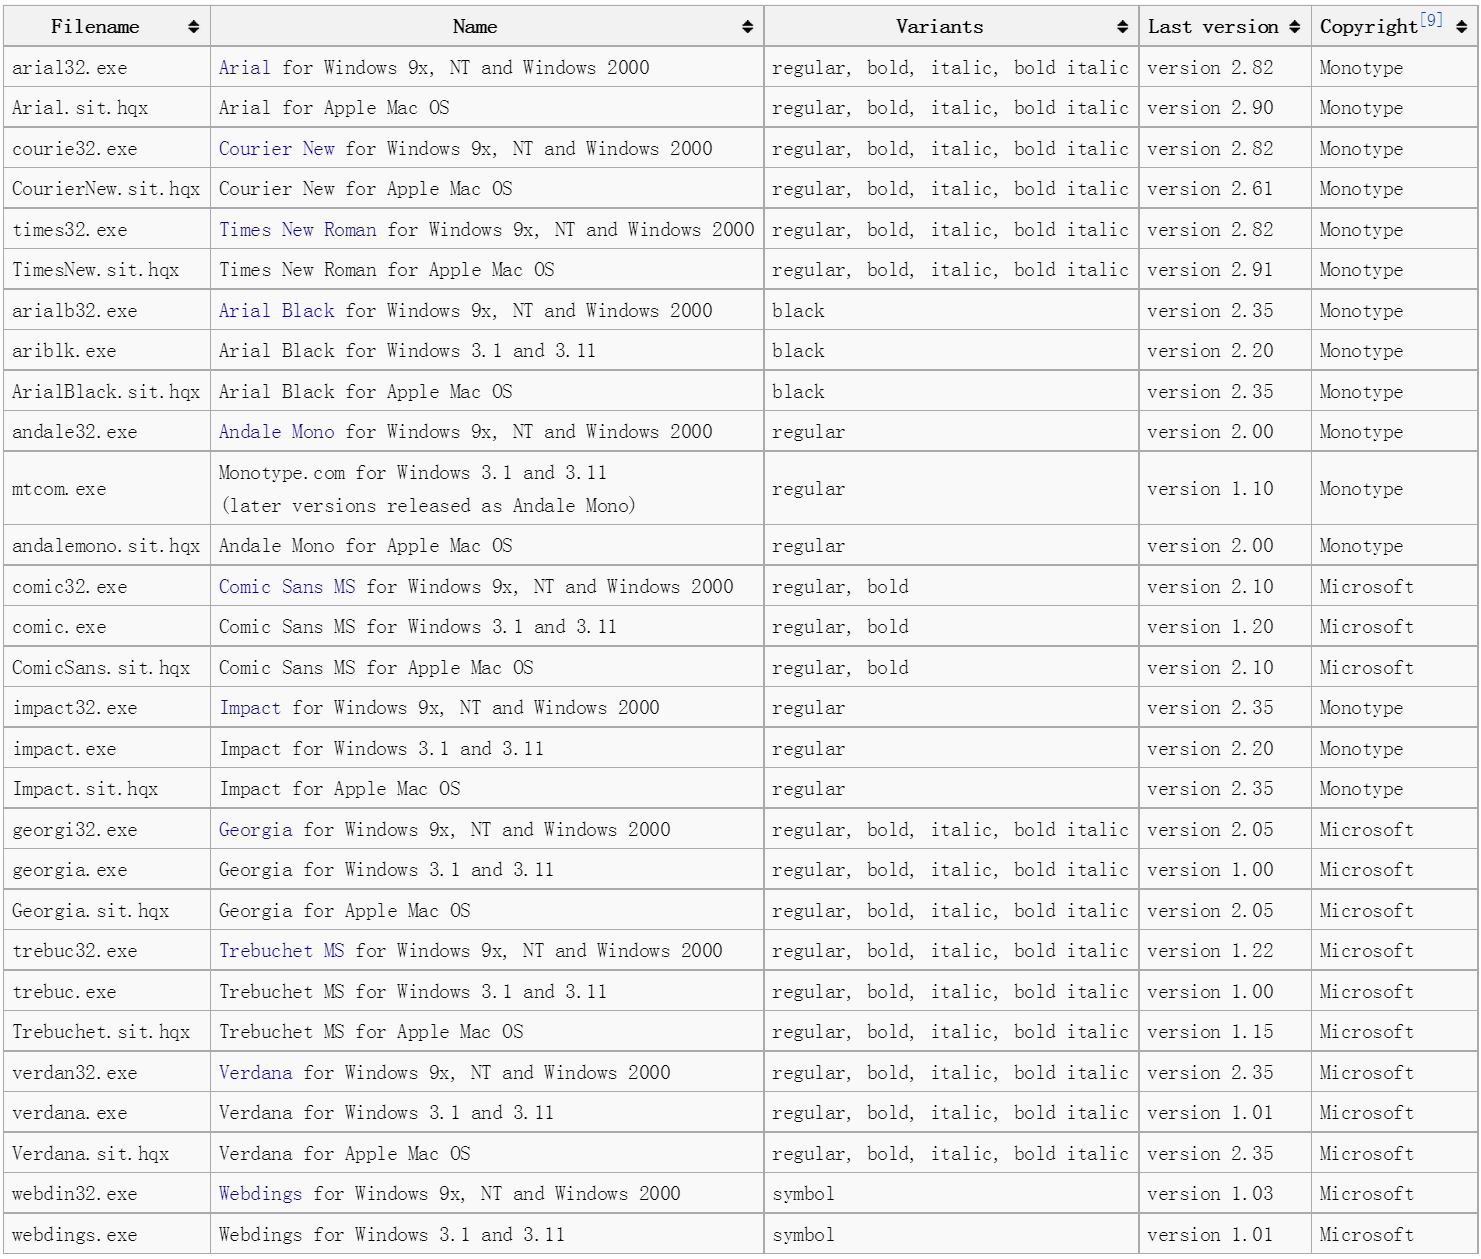
\includegraphics [width=1.3\textwidth]{cyt1.png} }
\caption{TrueType字型标准}
\label{cyt1}

\subsection{字体分析}

以下是对Web主流字体的分析。

	\subsubsection{Andale Mono} 	
~~~~~~	Internet Explorer 4.0的主流字体,现由Lucida Console替代。Arial

	\subsubsection{Arial} 
	
~~~~~~Arial是微软公司的网页核心字体之一,最常用的sans serif字体,其优点是支持正确打印并且便宜,Arial Black是Arial的变体,但是,当字号很小时不容易阅读并且当大写的“I”和小写的“l”无法区别时,可以使用Tahoma字体替代。
	
苹果系统没有Arial这种字体,但其对应有Helvetica字体,它是MAC机上与Arial 字体最相似的WEB字体,是一种非衬线字体\cite{cyt6}。
	
这也是Linux和Unix下的Web常用字体
	\subsubsection{Comic Sans MS} 
	
~~~~~~   类似手写,常用于纸本漫画及线上漫画(WebComic)以取代手写,风格类似于卡通式卖萌字体,但字体处理细节在“笔画均匀度”、“字间距”、“反锯齿”上处理不当。如\cite{cyt3}中作者David Kadavy所言,该字体并不适用于任何情况,只适合儿童使用。
	\subsubsection{Courier New} 
	
~~~~~~    Courier是等宽的粗衬线字体,因其等宽特性可以轻易对齐字段的左右边界,成为脚本和程序设计中源代码的常用字体[9],Courier New是Courier的变体,相对于Courier行距更宽。
	\subsubsection{Georgia} 
	
~~~~~~Georgia是一种衬线字体,具有小字下仍能清新辨识的特性,可读性很好。表面上,Georgia与Times New Roman相当类似,实质有很多不同。首先,在相同的字号下,Georgia的字元比Times New Roman的字元略大;其次,Georgia的字元线条较粗,衬线部分也比较钝而平。另外在数字部分也非常不同,Georgia采用称为“不齐线数字”的数字,特色在于数字会像西文字母般有高矮大小之别。
微软将Georgia列入网页核心字型,是视窗操作系统的内建字型之一。苹果电脑的麦金塔系统之后也跟进采用Georgia作为内建字型之一。
	
但是,数字“0”与字母“o”在Georgia字体下可能是显示成一模一样。
	\subsubsection{Impact} 
	
~~~~~~Impact是一个由设计师乔佛瑞•李在1965年发表的一个无衬线字体,笔画粗、间距紧以及内部空间狭窄,正如其名impact(压紧)所指。此字型的x字高相当大,几乎接近其大写字母的三分之二,因此升部相当短小,降部更是如此。因为字体较为粗犷,适合使用在Web页面标题上,而不常用在内文。
	\subsubsection{Times New Roman} 
	
~~~~~~    Times New Roman是Web开发最常用的的衬线字体之一,由于其中规中矩、四平八稳的经典外观,所以经常被选择为标准字体。《泰晤士报》首次采用了Times New Roman后,这个优秀的字型很快地博得了大众的青睐,获得了极大的成功,后来成为Web开发的重要字体之一。
	\subsubsection{Trebuchet MS} 
	
~~~~~~	 Trebuchet MS是一种无衬线字体,微软称Trebuchet MS为良好的网页设计字体,Trebuchet MS与其他常见的无衬线字体大不相同,其显著特色包括:大写字母“M”的两端与垂直线呈10度角;大写字母“Q”的尾巴;大写字母“A”中的横杠较低;小写字母“e”和数字“6、9”的尾巴较短;小写字母“g”的下圆带有开口;小写字母“i、j”上面的点为圆点;小写字母“l”的尾巴呈弯曲状;金钱符号“\$”的直竖笔画不贯穿S字母,只出现在上端和下端;“\&”符号是英文“Et”的合写;感叹号“!”下的点为圆点;斜体不单只是把原本字体倾斜,而是另外设计一套斜体的字母等。
   
	\subsubsection{Verdana} 
	
~~~~~~Verdana,无衬线字体,由于它在小字上仍有结构清晰端整、阅读辨识容易等高品质的表现,因而在1996年推出后即迅速成为许多领域所爱用的标准字型之一。
	\subsubsection{Verdana} 
	
~~~~~~Verdana,无衬线字体,由于它在小字上仍有结构清晰端整、阅读辨识容易等高品质的表现,因而在1996年推出后即迅速成为许多领域所爱用的标准字型之一。
    

\subsection{Web字体的基本特性}

在CSS中,Web字体相关的属性如Table \ref{tb1}所示

\begin{table}[h]
\centering
\begin{tabular}{lccc}  % {lccc} 表示各列元素对齐方式,left-l,right-r,center-c
\hline
font-family	 &font-size &font-weight &font-style\\         % \\ 表示重新开始一行
font-variant &font &text-decoration &text-transform\\        % & 表示列的分隔线
line-height &text-indent &text-align &vertical-align\\ 
letter-spacing & word-spacing & white-space & direction\\ \hline
\end{tabular}
\caption{Web字体属性列表}
\label{tb1}
\end{table}

\subsection{字体风格及使用场合}
从字体风格角度,字体主要包括Academic Categories及Popular Style \& Tags。如Figure \ref{cyt3}
所示

\makeatletter
\def\@captype{figure}
\makeatother
\centerline{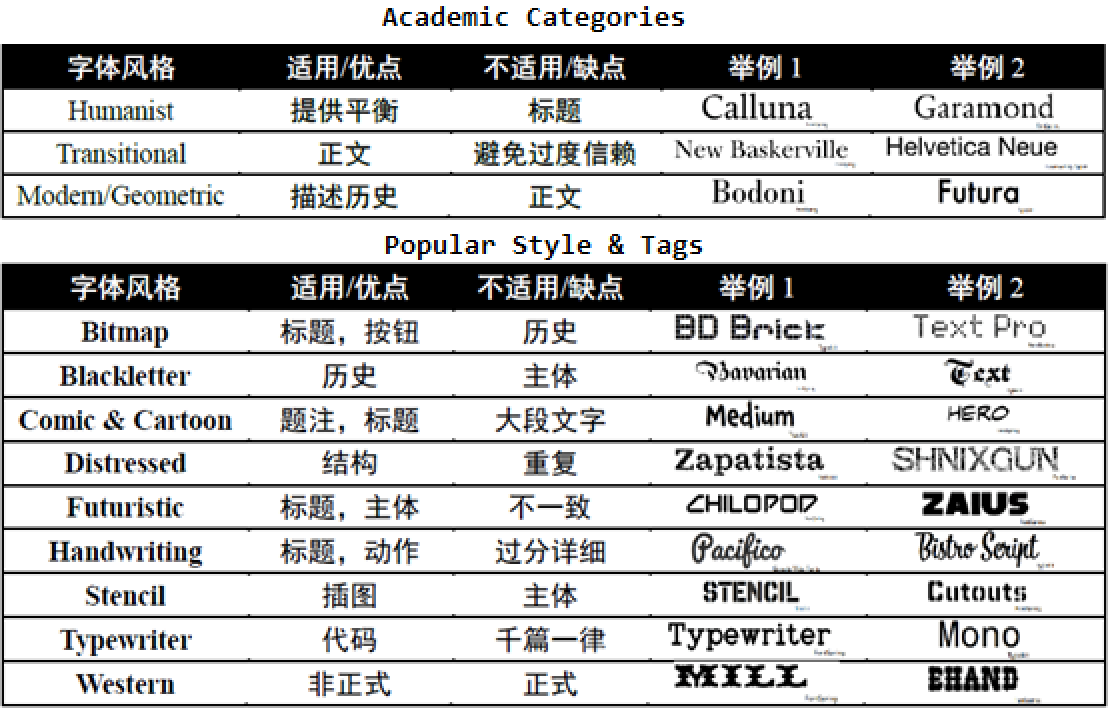
\includegraphics [width=1\textwidth]{cyt3.png} }
\caption{TrueType字型标准}
\label{cyt3}


\section{高细腻技术下的屏幕文字显示}
\subsection{术语解释}
\subsubsection{pt与px}

~~~~~~pt全称为point,即“磅”,是印刷行业的常用单位;px全称为pixel,即“像素”,是屏幕显示的基本单位。像素本身并没有确切的大小,而磅则是一个固定的长度单位,大小为1/72英寸。

\subsubsection{字体微调(font hinting)}
~~~~~~字体微调技术多见于TureType字体\cite{mxw1},是精确地定义字体所要显示的像素是一种方法,用以尽可能在小尺寸、低分辨率的情况下创建最好的字符位图形状。

TrueType字体使用矢量图形描述字符的轮廓,并在显示时在轮廓内进行填充,而字符在屏幕上实际显示时,又需要转化为一组像素点。在转化的过程中,矢量的轮廓往往无法紧密贴合像素点的边缘(见Figure \ref{mxw1})。此时若简单地对未被完全包括在轮廓内的像素进行二值化处理,显示效果将会与字体设计时的预期产生出入。在小字号中,这样的出入产生的出入将更为明显,并可能导致字符在屏幕上产生笔划粘连、残缺等问题(见Figure \ref{mxw2})。使用点阵字体是解决这一问题的最佳方案,因为点阵字体精确地控制了每一个像素的明暗,可以达到最佳的显示效果。然而,点阵字体通常为某一特定字号设计,不能将字号放大成为了其最大问题。在这样的背景下,字体的Hinting技术应运而生。Hinting的基本原理是在矢量字体中嵌入一些小字号的点阵字体,在字号较小时,直接将点阵结果显示在屏幕上;使用大字号时,再通过矢量图形进行渲染。Hinting技术有效地将点阵字体与矢量字体的优势融合起来,使得TrueType字体无论字号大小如何变化,都能在屏幕上清晰地显示出来。

\makeatletter
\def\@captype{figure}
\makeatother
\centerline{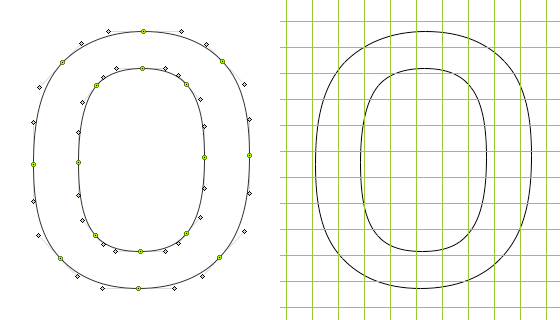
\includegraphics [width=0.7\textwidth]{mxw1.png} }
\caption{像素边缘未被矢量轮廓贴合示意图\cite{mxw2}}
\label{mxw1}

\makeatletter
\def\@captype{figure}
\makeatother
\centerline{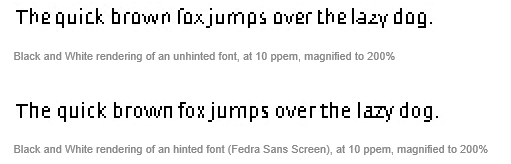
\includegraphics [width=1\textwidth]{mxw2.png} }
\caption{黑白渲染模式下使用Hinting技术使显示效果产生差异}
\label{mxw2}



\subsubsection{DPI}
~~~~~~DPI全称为dots per inch,即每英寸容纳、打印或显示的点的数目,最初被应用于印刷行业。DPI越大,通常意味着输出越精细,输出效果也就越好。尽管在显示器上,像素才是最终的输出对象,但DPI的称呼并未相应地产生变化,原因在于PPI(pixels per inch)已被约定俗成地用于衡量图像的采样率,成为了输入层面的度量值。近年来,在度量显示器显示画面的精细程度时也会使用PPI,但此时,DPI和PPI可以被认为是同一概念的不同称呼。
\subsection{高DPI与高分辨率}
~~~~~~分辨率决定了屏幕上所能显示的像素数量多少。由于任何网页内容最终都被转化为像素进行输出,分辨率也就决定了能够显示的网页元素的多少,分辨率越高,一屏幕能够容纳的内容也就越多;又由于像素本身没有大小的概念,分辨率也就无法决定网页元素显示的大小。DPI的大小则不同。DPI的数值体现了像素的密度水平,像素密度越大,显示单位物理长度内容使用的像素数目就越多,显示效果也就越精细。

这里需要说明的是,DPI的提高并不是总能改善显示效果的。一旦DPI突破人眼极限,再高的技术指标也不能影响画面的显示效果。根据苹果公司于第三代iPad发布会上给出的Retina设计标准公式,在通常的使用距离下,手机的像素密度达到300DPI,平板电脑的像素密度达到260DPI,PC与笔记本电脑的像素密度达到200DPI之后,人眼就无法再区分出单个像素点,画面也就不会再出现颗粒感。

现代显示器的分辨率与DPI并不是同步发展的。从Table \ref{tb2} 中,我们可以看出,在小尺寸4K分辨率显示器问世之前,主流的家用显示器,DPI数值都在100左右。

\begin{table}[h]
\centering
\begin{tabular}{lccc}  % {lccc} 表示各列元素对齐方式,left-l,right-r,center-c
\hline
尺寸与分辨率 & PPI \\\hline
19寸1440×900 & 90 \\
21.5寸1920×1080 & 102 \\
23寸1920×1080 & 96 \\
24寸1920×1200  & 94 \\
27寸1920×1080 & 82 \\
27寸2560×1440 & 109 \\
29寸2560×1080 & 96 \\
28寸3840×2160 & 157 \\
32寸3840×2160 & 127\\ \hline
\end{tabular}
\caption{主流显示器尺寸PPI对照表}
\label{tb2}
\end{table}

\subsection{高DPI下的屏幕文字可读性改进技术}
~~~~~~文字的可读性最终体现在阅读给人眼带来的疲劳感上。无论应用怎样的可读性改进技术,只要能有效地降低人阅读屏幕显示文本的疲劳感,延长用户从开始阅读到被迫离开设备休息的时间,就都是成功的。应用这些可读性改进技术后,网页设计就获得了更大的自由度。在低分辨率、低DPI时代,为了保证文字的可读性,网页设计者往往倾向于使用一些较粗的字体,但从以目前的分辨率,在一般的DPI下,使用比以往更细的字体仍然能实现同样清晰、优雅的文字显示效果。

\textbf{\large Font Hinting}:不可否认,字体微调技术在低分辨率、小尺寸屏幕的时代非常有效。然而,随着分辨率和DPI数值的提升,TrueType字体的Hinting技术虽然仍有效果,但效果已不十分明显。一方面,高分辨率和高DPI使得显示同样实际大小的字符时,可以进行渲染的像素数目大幅增加,不使用Hinting已经可以达到良好的显示效果;另一方面,由于目前并没有有效的自动化Hinting工具,字符的微调需要设计师的人工控制。有数据显示,即使只对256个ASCII字符进行二值化微调,一名有经验的设计师也需要工作80小时\cite{mxw3}。因此,Hinting技术在高DPI时代已然成为鸡肋,吃力不讨好,只有在与其它显示技术结合的情况下,Hinting才能重新发挥其应有的作用。

\textbf{\large ClearType\&DirectWrite}: ~ClearType技术是针对LCD显示设备开发的平滑显示技术。与CRT显示器不同,LCD显示设备中的一个像素可以被分解为3个次像素,分别显示红、绿、蓝三种颜色。基于人眼的视觉系统对颜色的细节错误不敏感,而对亮度的细节错误更敏感的事实,ClearType技术在字符边缘使用一些彩色像素点来增强显示效果\cite{mxw4}。(ClearType技术的简单实现机制见Figure \ref{mxw3}。

DirectWrite技术与ClearType类似,不同之处在于,ClearType技术只在水平方向平滑的字符边缘的显示效果,而DirectWrite技术在水平和垂直两个方向都能使字符的显示更加平滑。
需要说明的是,ClearType与DIrectWrite技术只对拥有Hinting信息的字体产生效果。

~~

\makeatletter
\def\@captype{figure}
\makeatother
\centerline{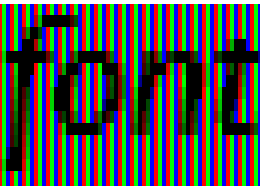
\includegraphics [width=0.4\textwidth]{mxw3.png} }
\caption{LCD显示屏像素点极度放大后的ClearType显示效果}
\label{mxw3}

\textbf{\large Retina}:~工作方式与游戏中常见的抗锯齿技术十分类似。以MacBook Pro with Retina Display为例,工作时,显卡渲染出2880×1800的像素,然后以四个像素为一组,输出显示器上一个实际的像素。这样,用户所看到的文字、图像大小与实际使用1440×900分辨率时的保持一致,但精细度得到了明显的提高。


\subsection{不同情况下的字体显示情况}

\subsubsection{Font Hinting}

~~~~~~在前文中,字体微调在二值渲染模式下的显示效果已经得到了展示。此处将展示字体微调技术在灰度渲染模式下产生的效果。
灰度渲染模式将未被TrueType字体的轮廓全部包围的像素以一定亮度的灰色进行填充,可以避免简单的黑白渲染带来的字符残缺问题,但字符粘连的问题仍然不能有效解决。从Figure \ref{mxw4}~中可以看出,在不使用Hinting技术时,小字号的文字整体发虚,势必加剧用眼疲劳;使用Hinting技术后,字符的主干部分黑色更深,文字显得更“实”,给用户带来了更好的阅读体验。

\makeatletter
\def\@captype{figure}
\makeatother
\centerline{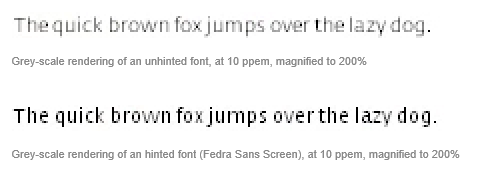
\includegraphics [width=1\textwidth]{mxw4.png} }
\caption{灰度渲染模式下Hinting技术造成的显示效果差异}
\label{mxw4}

\subsubsection{ClearType\&DirectWrite}

~~~~~~如Figure \ref{mxw5}~所示,开启ClearType技术后,文字周边的锯齿状轮廓几乎不可见,边缘更加平滑。之所以在放大的状态下,开启ClearType后的文字显得发虚,是因为ClearType技术对次像素的处理经过图像放大的插值计算后产生了一些负面效果,在原大小下,文字边缘仍然是清晰的。

\makeatletter
\def\@captype{figure}
\makeatother
\centerline{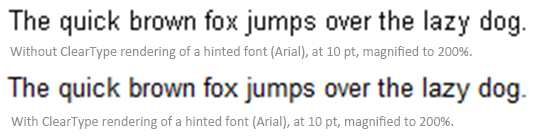
\includegraphics [width=1\textwidth]{mxw5.png} }
\caption{ ClearType技术造成的显示效果差异}
\label{mxw5}

\subsubsection{Retina}
~~~~如Figure \ref{mxw6},左右的对比结果显然。在某非Retina设备中,图标和文字周边的像素点与锯齿十分明显,而在相同实际物理大小的情况下,搭载了Retina技术的iPad显示效果则相当出彩,图标和文字的边缘都十分平滑,以肉眼无法察觉出像素点的存在。

~~

\makeatletter
\def\@captype{figure}
\makeatother
\centerline{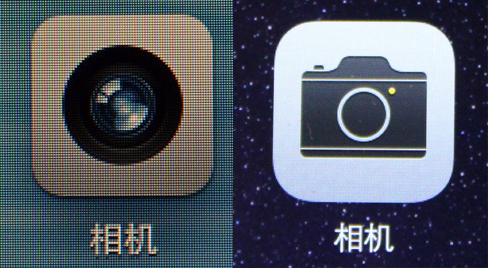
\includegraphics [width=0.6\textwidth]{mxw6.png} }
\caption{ 非Retina与Retina显示设备的显示效果对比}
\label{mxw6}

\section{Web应用字体使用建议}

~~~~~~基于以上分析,结合\cite{lj1}中的讨论,我们提出了Web应用字体选择的建议。

\subsection{善于使用字体组合}

~~~~~~使用不同字体的组合可以让文本的差异性给用户带来更好地体验,无论是从逻辑上更容易分类,还是从视觉上更方便感知内容角度,字体组合都是非常重要的一个设计方法。关于字体组合有以下几条建议:

\begin{itemize}
	\item 避免相似性产生的冲突
	如Figure \ref{Jing_fig1} 相似的但是又有区别的字体放在同一块区域,尤其是在大小一致的情况下,很容易彼此造成干扰,产生不好的视觉体验,可能导致认知困难。因为人眼需要花费额外精力去区别两者,这一点要避免。

\makeatletter
\def\@captype{figure}
\makeatother
\centerline{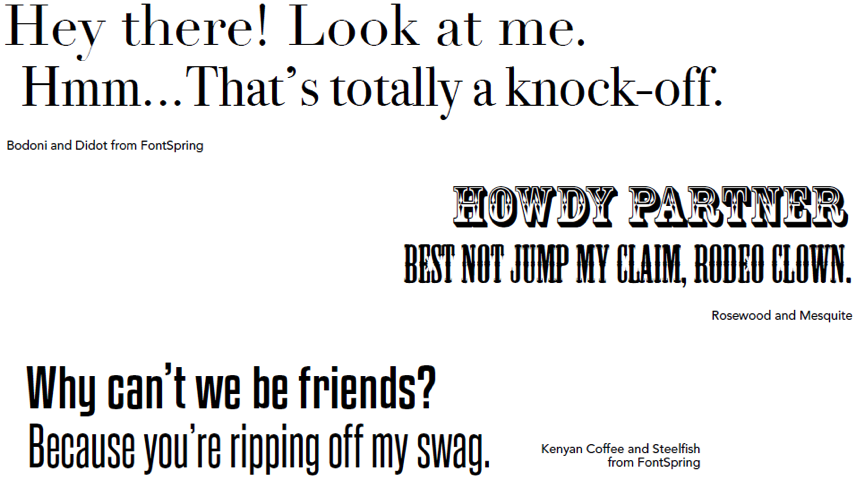
\includegraphics [width=0.6\textwidth]{Jing_fig1.png} }
\caption{ 相似字体产生冲突}
\label{Jing_fig1}	
	
	\item 朴素与时尚兼具
	
	适度使用一些时尚的字体,可以使得文本具有更强的吸引力,但是也同时要结合简朴的字体,正所谓淡妆浓抹总相宜,达到一种简朴和时尚的平衡会是一个很好的选择,如下Figure \ref{Jing_fig2} 。
	
\makeatletter
\def\@captype{figure}
\makeatother
\centerline{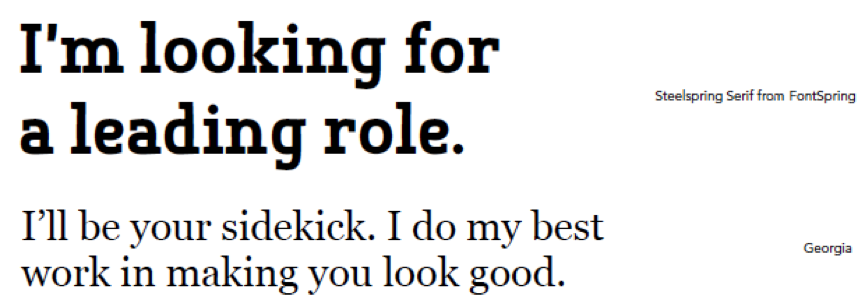
\includegraphics [width=0.8\textwidth]{Jing_fig2.png} }
\caption{朴素与时尚结合示例 }
\label{Jing_fig2}

	\item 不要忘记使用斜体
	
	斜体是一种简单的变换,但往往得到不错的效果,其接近手写体的风格,对文本有一定强调作用,也增强了文本的艺术性,例如 Figure \ref{Jing_fig3}~所示。
	
\makeatletter
\def\@captype{figure}
\makeatother
\centerline{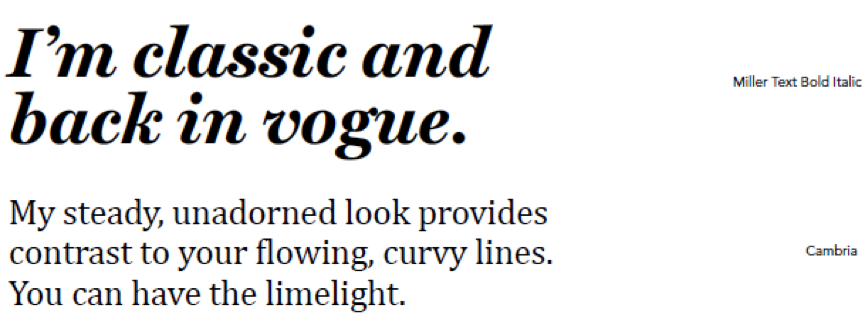
\includegraphics [width=0.8\textwidth]{Jing_fig3.png} }
\caption{斜体的使用 }
\label{Jing_fig3}
	\item 标题与正文不同
	
	对于标题和正文采用不同的风格可以有效的突出标题,使用户很容易的得到关键内容,而且在保证文本整体一致性(正文)的基础上丰富了文本的视觉体验。如Figure \ref{Jing_fig4}~所示。
	
\makeatletter
\def\@captype{figure}
\makeatother
\centerline{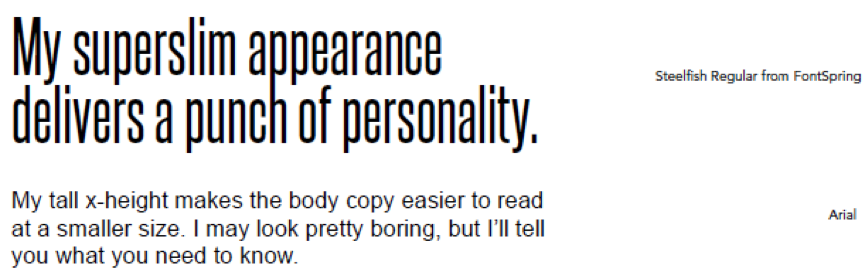
\includegraphics [width=0.8\textwidth]{Jing_fig4.png} }
\caption{斜体的使用 }
\label{Jing_fig4}
	
\end{itemize}

\subsection{利用对比反差建立字体层次}

\subsubsection{列出需要表达的所有层次的信息}

~~~~~~Web网页设计中往往有以下的信息块以展现字体。他们的功能不同,往往对应于不同的信息层次,利用字体层次分别对应不同的信息层次是一种比较好的处理办法。常见的信息块包括:
\begin{itemize}
\item Navigation (导航)
\item Headline (标题)
\item Sub-Headline for main content (正文的副标题)
\item Introductory (引言)
\item Sidebar headline (边栏标题)
\item Sidebar body copy (边栏正文)
\item Link text (链接文本)
\item Call to action (操作提示)
\item Contact information (联系信息)
\item Footer links (下边栏链接)
\end{itemize}
\subsubsection{基于不同信息层次的字体对比处理}

~~~~~~对于不同的信息层次采用不同的字体,有两种思路一是使用尺寸、颜色、粗细和形状产生对比,如Figure \ref{Jing_fig5}~二是对特定的数据元素使用差异化字体,如\ref{Jing_fig6}。

\makeatletter
\def\@captype{figure}
\makeatother
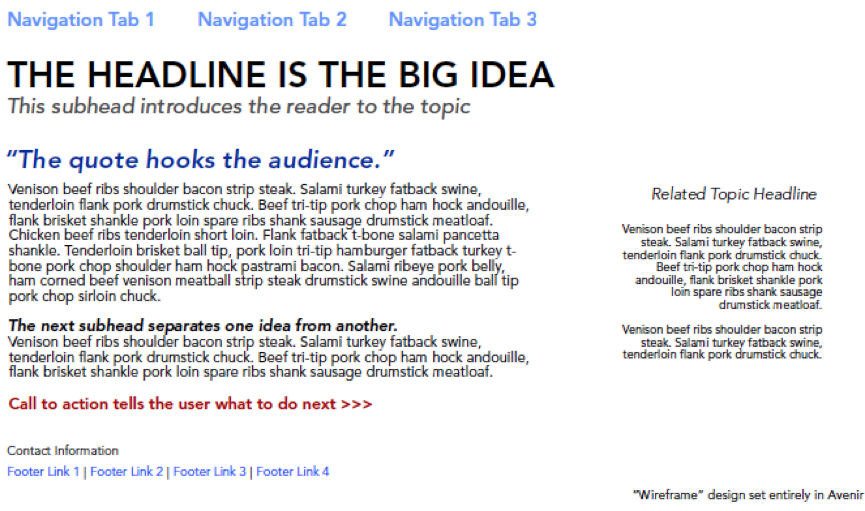
\includegraphics [width=0.8\textwidth]{Jing_fig5.png} 
\caption{字体层次化差异处理示例一}
\label{Jing_fig5}

\makeatletter
\def\@captype{figure}
\makeatother
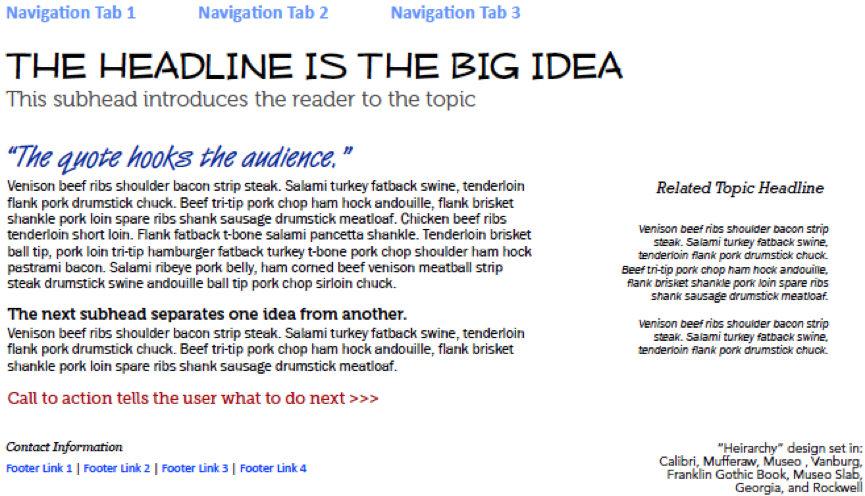
\includegraphics [width=0.8\textwidth]{Jing_fig6.png} 
\caption{字体层次化差异处理示例二}
\label{Jing_fig6}

\subsection{处理难以完全控制的情况}

~~~~~~设计者需要意识到,无论怎样进行设计,Web页面最终需要在客户端的浏览器上展现效果,字体的选择很多情况下因此不能起到决定性的作用,反而是客户端的操作系统环境和浏览器配置占据了较大的比重。

\subsubsection{浏览器和操作系统的字体支持}
	
	~~~~~~Figure \ref{Jing_browser}~中显示了2014年全年各个浏览器的市场份额,Figure \ref{Jing_fig10}~给出了主流浏览器对字体的支持情况。时至今日,依旧没有一个对于各个浏览器的一个统一而足够优雅的字体选择解决方案,因此设计者在字体设计过程中,需要更多的考量浏览器对字体的支持情况以及不同操作系统之间字体的差异性。

\makeatletter
\def\@captype{figure}
\makeatother
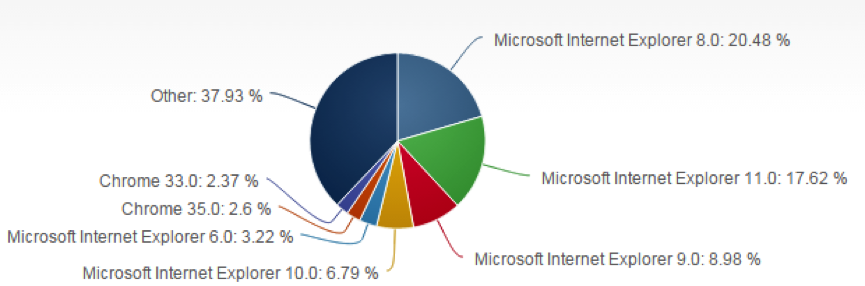
\includegraphics [width=1\textwidth]{Jing_fig7.png} 
\caption{2014-2015各个浏览器市场份额}
\label{Jing_browser}

\makeatletter
\def\@captype{figure}
\makeatother
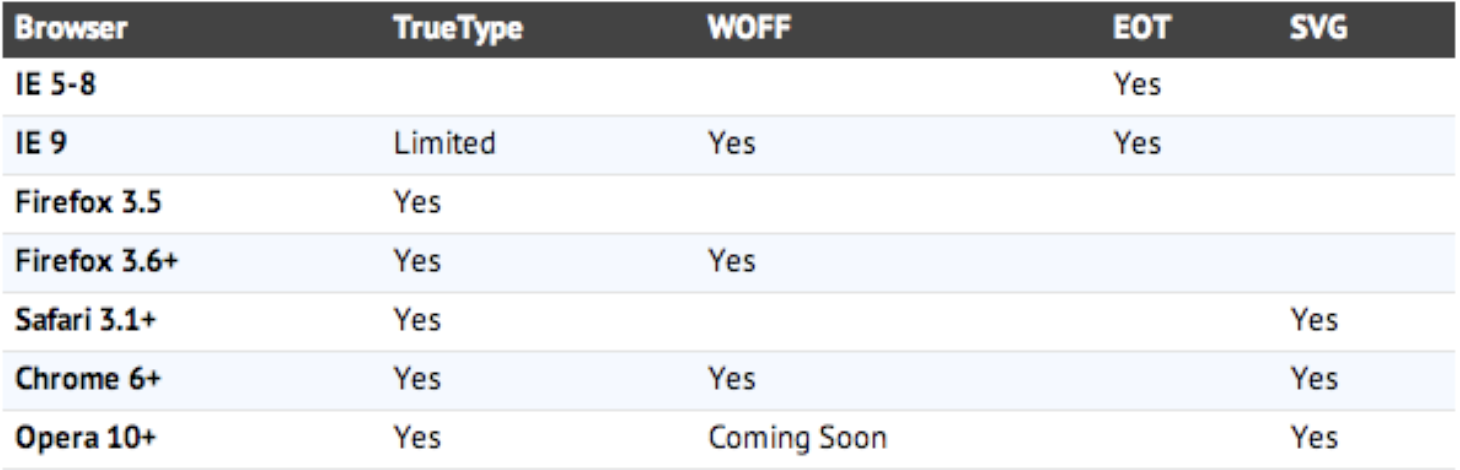
\includegraphics [width=1\textwidth]{Jing_fig10.png} 
\caption{主流浏览器对字体的支持情况}
\label{Jing_fig10}

\subsubsection{ Web安全字体}

~~~~~~基于兼容性的考虑,可以选择使用对所有主流操作系统支持的字体集合,这样可以在字体显示发那个面提供较好的安全性,缺点是会在显示效果方面有一定的牺牲。

截止到2011年的19种Web安全字体包括,Arial, Arial Black , Arial Narrow. Verdana, Georgia, Times New Roman, Trebuchet MS, Courier, Courier New, Impact, Comic Sans MS, Tahoma, Lucida Sans Unicode, Garamond, MS Sans Serif, MS Serif, Palatino Linotype, Symbol, Bookman Old Style。

\subsubsection{ 使用@font-face}

~~~~~~Bulletproof @font-face语法以及进阶版Footspring @font-face语法,用于诱导浏览器使用它们支持的最佳的(或者某些情况下唯一的)web字体格式。
写法如下所示

\makeatletter
\def\@captype{figure}
\makeatother
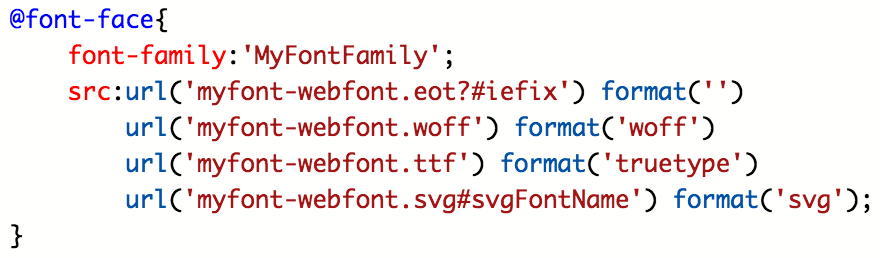
\includegraphics [width=0.9\textwidth]{Jing_fig11.png} 
\label{Jing_fig11}

\subsubsection{字体尺寸控制}
		\begin{itemize}
			\item 描述尺寸的标准有如下几种:
			\begin{itemize}
			\item 绝对尺寸关键字:包括xxx-small, x-small, small, large, x-large and xx-large.
			\item em:衡量宽高(尤其是高度),em-square标准是基于字体设计的(也叫做
		em-box)
			\item 相对尺寸关键字:larger和smaller。基于父对象的尺寸进行变化。
			\item 比例关键字:一种较为可靠的使用比例描述文本尺寸的方法。
			\end{itemize}
			\item 对于字体尺寸的控制,建议是结合比例和em作为标准使用。具体是\cite{nutshell}中所指出的方法,在正文中使用比例关键字使body部分的文本轻微缩小,当设计者想使一些独立文本比周围文本偏大的情况下,使用em。例子如下
		\end{itemize}
			
\makeatletter
\def\@captype{figure}
\makeatother
\centerline{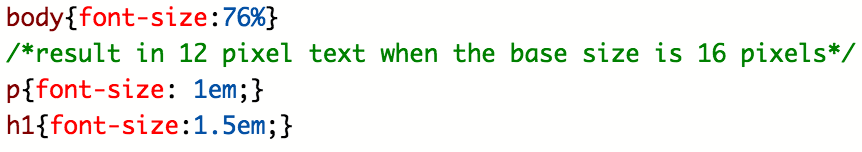
\includegraphics [width=0.8\textwidth]{Jing_fig9.png} }
\label{jing9}

\subsubsection{创建理想的字体栈}

~~~~~~浏览器将会从左到右地寻找字体直到它找到一个用户计算机中存在的字体。比如它会查找Georgia字体,如果没有找到,它将会查找Times字体等等。需要注意的时同一个字体栈下的所有字体应该有相同的(或相似的)高宽比。设计者还需要确保考虑了不同的操作系统。同时需要有大量的备选字体以供浏览器最终可以找到能够满足的字体。
	


\subsection{测试实际效果}

~~~~~~设计者的设计结果最终要在用户的浏览器上展示效果,所以需要再设计时进行充分的测试,充分掌握选择的字体,以及字体栈中的替代字体可能产生的表现。

\bibliographystyle{plain}
\bibliography{Web_fonts}

\end{document}
